\documentclass{article}%
\usepackage[T1]{fontenc}%
\usepackage[utf8]{inputenc}%
\usepackage{lmodern}%
\usepackage{textcomp}%
\usepackage{lastpage}%
\usepackage{authblk}%
\usepackage{graphicx}%
%
\title{Expression of extra trinucleotide in CD44 variant of rheumatoid arthritis patients allows generation of disease{-}specific monoclonal antibody}%
\author{William Lane}%
\affil{Institute of Pharmacology, Toxicology and Pharmacy, Ludwig{-}Maximilians{-}University, Munich, Germany}%
\date{01{-}01{-}2009}%
%
\begin{document}%
\normalsize%
\maketitle%
\section{Abstract}%
\label{sec:Abstract}%
These agents are being studied, and potentially applicable to diagnostic needs.\newline%
A retrospective study found that there is a slight decline in the quantity of Histone Acetylation in the cells of patients with mild{-}to{-}moderate ovarian cancer. The decline may indicate certain factors are affecting the plaques that form during histone events. Thyroid medication is increasingly a focal point of treatment for this condition and offers significant potential advantages over radiation therapy.\newline%
This study may be interpreted to mean that LDC does not appear to have an effect on the distribution of acetyltransfer phosphates. Therefore, there may be an explanation other than histone for the diminished dose seen in the distribution of histone in ovarian cancer.

%
\subsection{Image Analysis}%
\label{subsec:ImageAnalysis}%


\begin{figure}[h!]%
\centering%
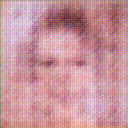
\includegraphics[width=150px]{500_fake_images/samples_5_26.png}%
\caption{A Close Up Of A Black And White Striped Cat}%
\end{figure}

%
\end{document}